% Standalone TikZ figure. Compile: figc thisfile.tex  →  out/thisfile.{pdf,png}
% In the thesis: \includegraphics{figures/out/thisfile.pdf}
\documentclass[tikz,border=2pt]{standalone}
\usepackage{amsmath,amssymb}
% Match the thesis body font so the figure does not look pasted in.
% \usepackage{newtxtext,newtxmath}   % Times-like
% \usepackage{lmodern}               % Computer Modern (default LaTeX look)
\usetikzlibrary{arrows.meta,positioning,fit,backgrounds,calc,shapes.geometric}

% One palette, defined once, reused by every figure in the thesis.
\definecolor{accent}{HTML}{2F5D8C}
\definecolor{accentbg}{HTML}{E8EFF6}
\definecolor{muted}{HTML}{6B7280}

\tikzset{
  box/.style   = {draw=accent, fill=accentbg, rounded corners=2pt,
                  align=center, inner sep=5pt, minimum height=8mm,
                  font=\small},
  ghost/.style = {draw=muted, fill=white, rounded corners=2pt, align=center,
                  inner sep=5pt, minimum height=8mm, font=\small},
  flow/.style  = {draw=accent, -{Stealth[length=2mm]}, thick},
  lbl/.style   = {font=\scriptsize, inner sep=2pt, fill=white},
}

\begin{document}
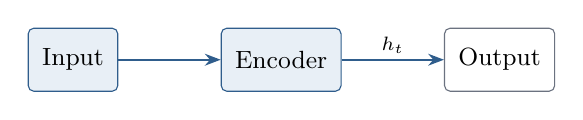
\begin{tikzpicture}[node distance=7mm and 13mm]
  \node[box]                        (in)  {Input};
  \node[box,  right=of in]          (enc) {Encoder};
  \node[ghost,right=of enc]         (out) {Output};

  \draw[flow] (in)  -- (enc);
  \draw[flow] (enc) -- node[lbl,above] {$h_t$} (out);
\end{tikzpicture}
\end{document}
